\documentclass[12pt, letterpaper, twoside]{article}
\usepackage{graphicx}
\usepackage[utf8]{inputenc}
\usepackage{longtable}

\title{AI607 Homework 1 Report}
\author{20214487 Geonju Lee}
\date{}

\begin{document}

\maketitle

\section{In-degree and Out-degree}

\begin{center}
% \begin{tabular*}{\textwidth}{ c c }
\begin{longtable}{ c c }  
    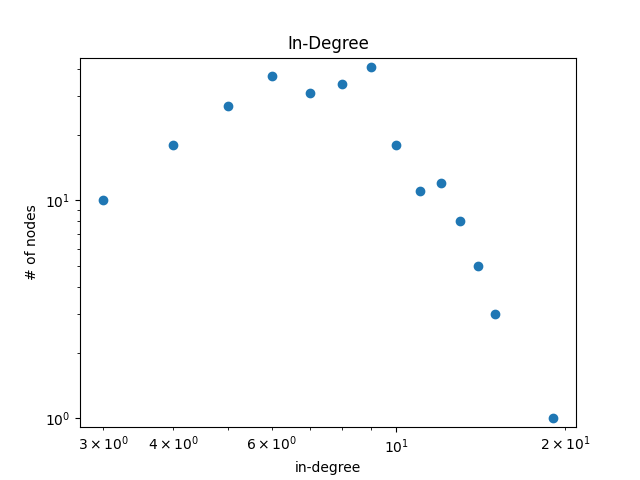
\includegraphics[width=0.5\textwidth]{1S_indeg.png} 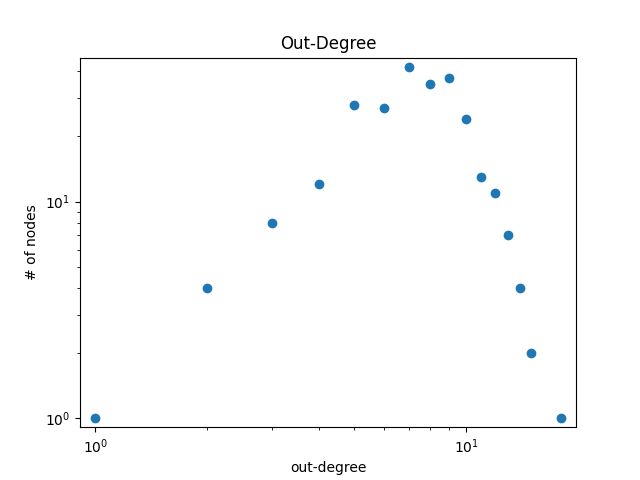
\includegraphics[width=0.5\textwidth]{1S_outdeg.png} \\
    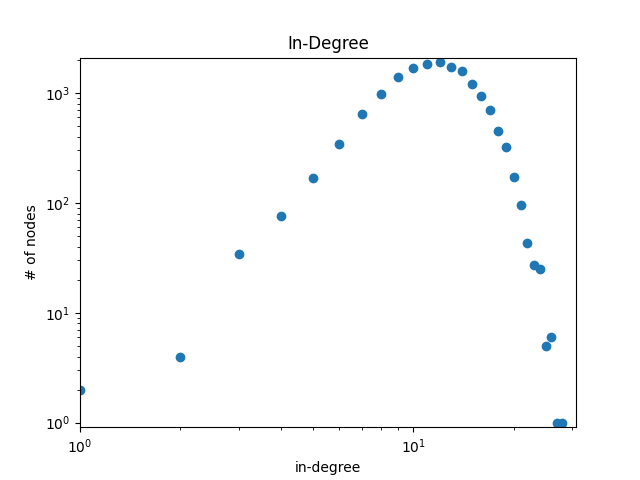
\includegraphics[width=0.5\textwidth]{1L_indeg.png} 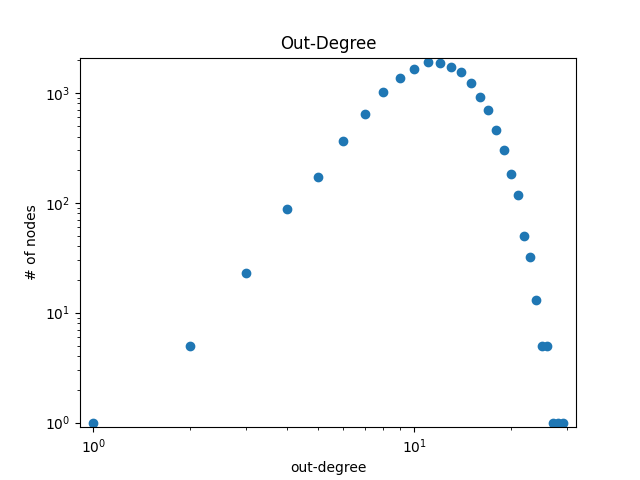
\includegraphics[width=0.5\textwidth]{1L_outdeg.png} \\
    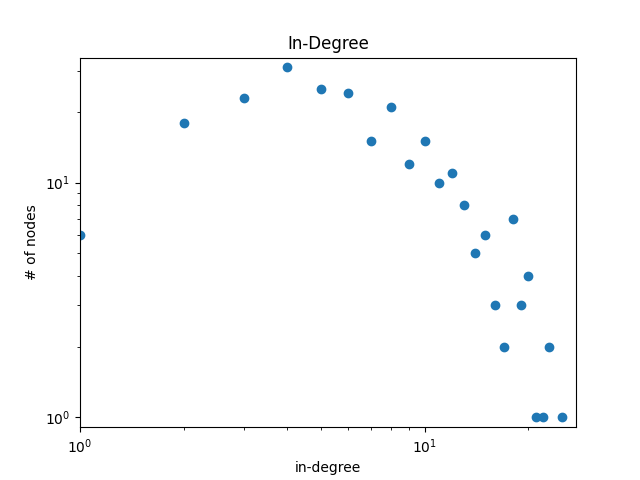
\includegraphics[width=0.5\textwidth]{2S_indeg.png} 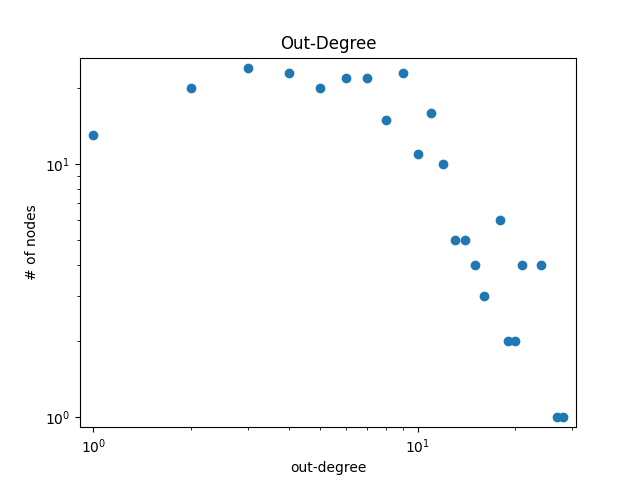
\includegraphics[width=0.5\textwidth]{2S_outdeg.png} \\
    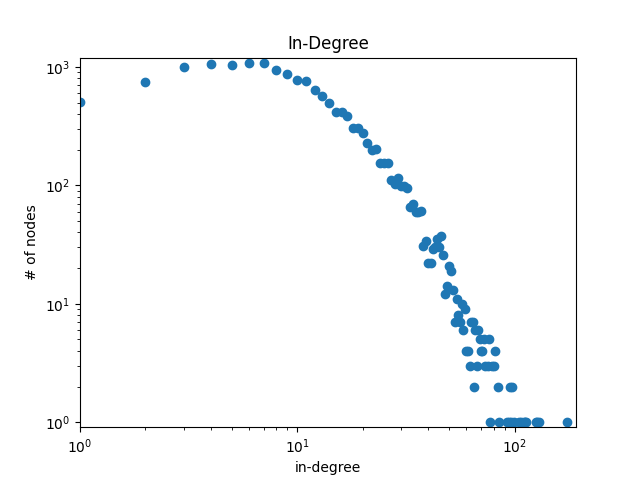
\includegraphics[width=0.5\textwidth]{2L_indeg.png} 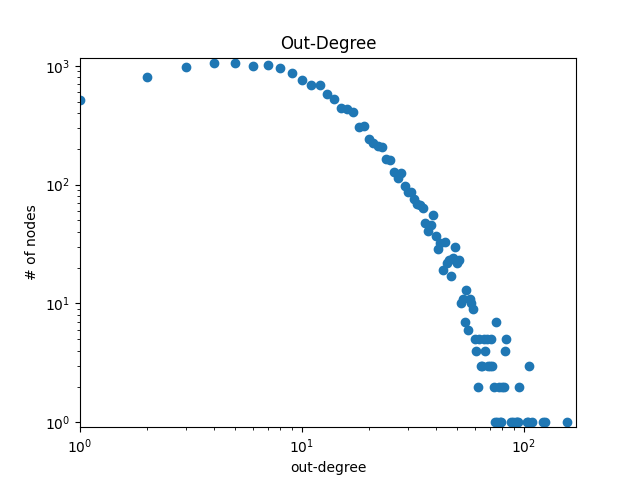
\includegraphics[width=0.5\textwidth]{2L_outdeg.png} \\
    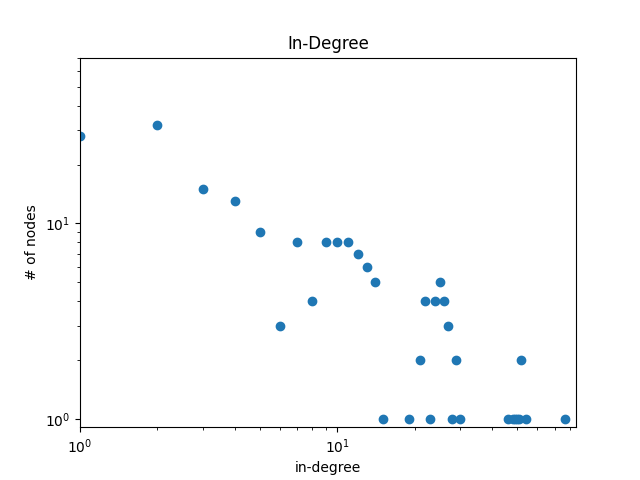
\includegraphics[width=0.5\textwidth]{3S_indeg.png} 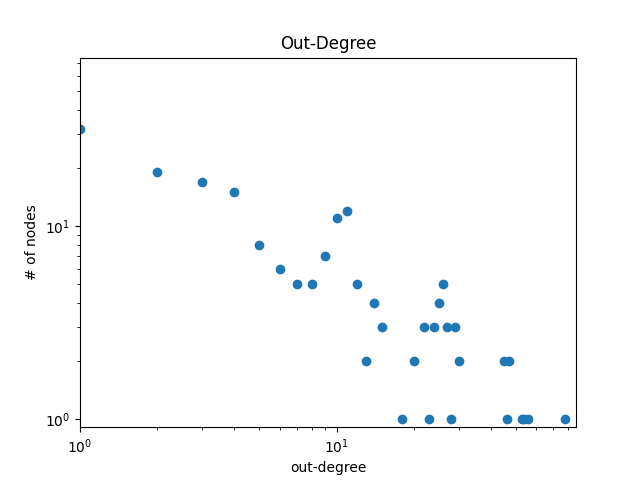
\includegraphics[width=0.5\textwidth]{3S_outdeg.png} \\
    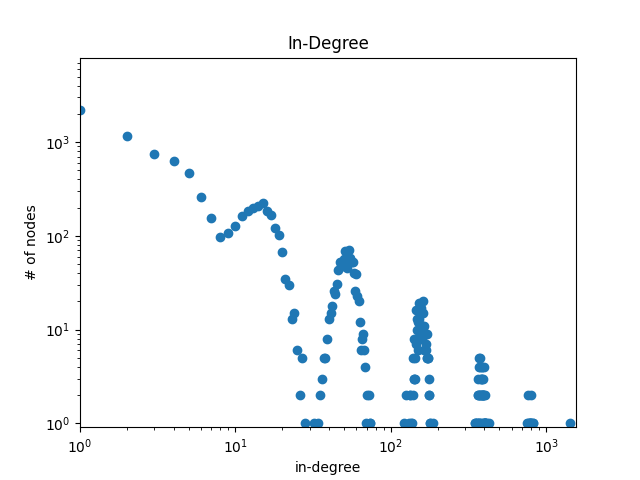
\includegraphics[width=0.5\textwidth]{3L_indeg.png} 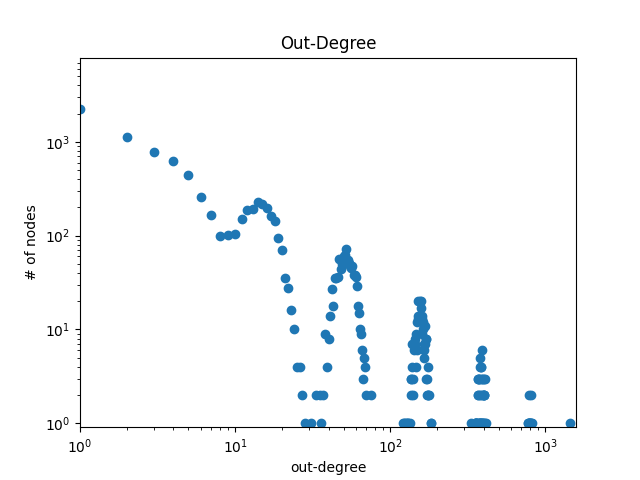
\includegraphics[width=0.5\textwidth]{3L_outdeg.png} \\
\caption{Plots of the in- and out- degree distributions of $G_{1,S}$, $G_{1,L}$, $G_{2,S}$, $G_{2,L}$, $G_{3,S}$ and $G_{3,L}$ from top to bottom; in-degree plots on the left side and out-degree plots on the right side.}
\end{longtable}
% \end{tabular*}

\end{center}

\section{Singular values}

\begin{center}
    % \begin{tabular*}{\textwidth}{ c c }
    \begin{longtable}{ c c }  
        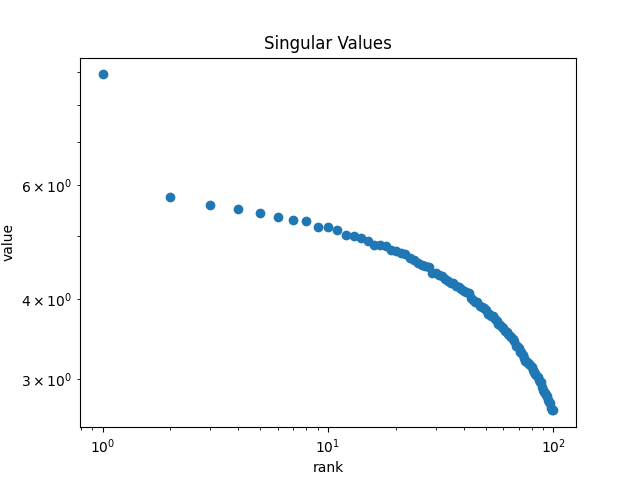
\includegraphics[width=0.5\textwidth]{1S_svd.png} 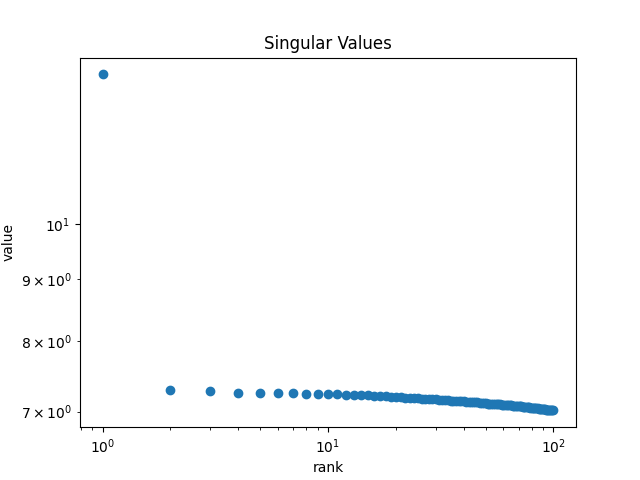
\includegraphics[width=0.5\textwidth]{1L_svd.png} \\
        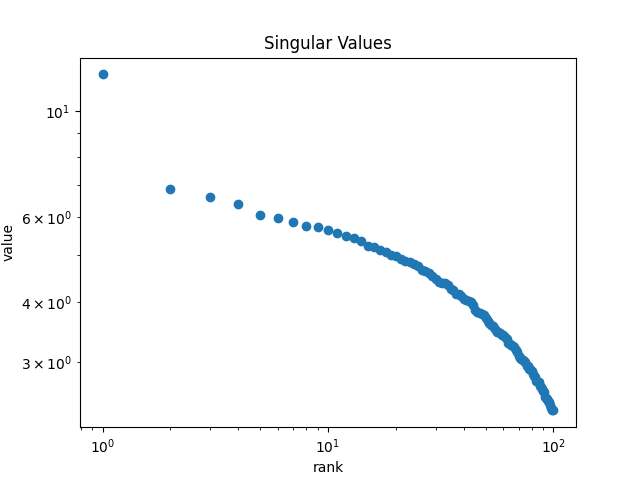
\includegraphics[width=0.5\textwidth]{2S_svd.png} 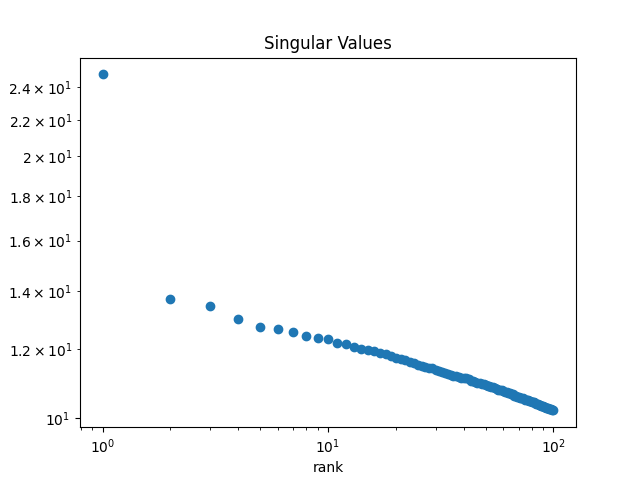
\includegraphics[width=0.5\textwidth]{2L_svd.png} \\
        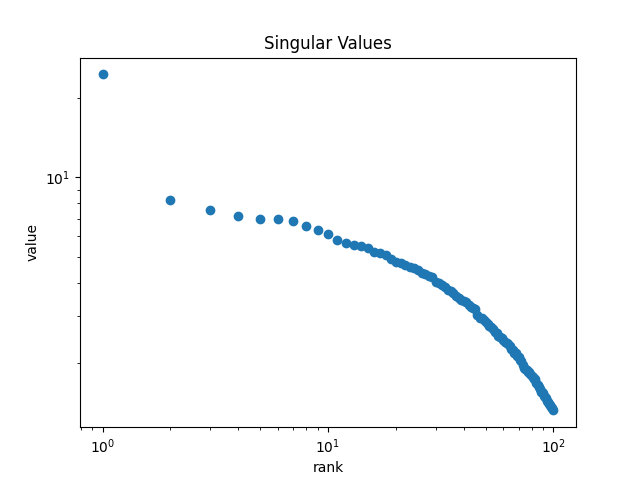
\includegraphics[width=0.5\textwidth]{3S_svd.png} 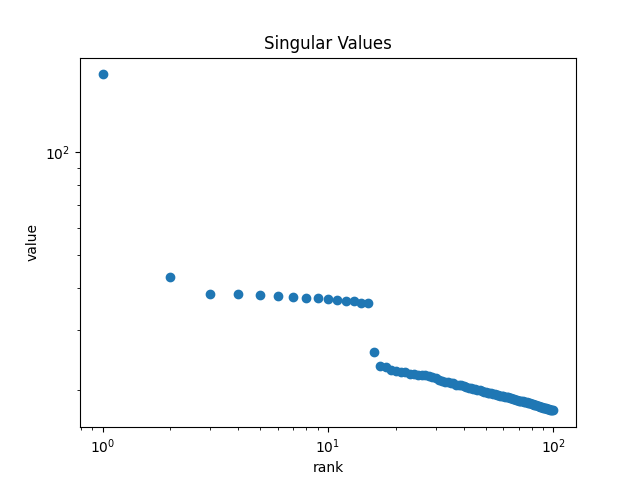
\includegraphics[width=0.5\textwidth]{3L_svd.png} \\
    \caption{Plots of the singular values of $G_{1,S}$, $G_{1,L}$, $G_{2,S}$, $G_{2,L}$, $G_{3,S}$ and $G_{3,L}$ from left to right, and from top to bottom}
    \end{longtable}
    % \end{tabular*}
    
    \end{center}

\section{Analysis}

For S1, the degree distribution is just a simple normal distribution, since $p_a,p_b,p_c,p_d$ are equal. For S2, the degree distribution seems to follow the power law.
For S3, the degree distribution roughly follows the power law, however, it fluctuates severely, having some 'peaks' in the distribution.
This is because, as the probabilities differ, the expected degrees differ exponentially.

In terms of component size, since the ratio between the numbers of nodes and edges are large (for 'small' graphs, $N=256$, $E=2,000$, and for 'large' graphs, $N=16,384$, $E=200,000$), the graphs are likely to have a giant component that contains most of the $N$ nodes.
To be more specific, $G_{1,S},G_{1,L}$, simple random graphs will have edges equally distributed over nodes, while $G_{3,S},G_{3,L}$, kronecker graphs with unbalanced probability over the quadrants, are likely to have 'core-periphery' structure.
\end{document}